%%%%%%%%%%%%%%%%%%%%%%%%%%%%%%%%%%%%%%%%%%%%%%%%%%%%%%%%%%%
\documentclass[dvipdfmx]{jlreq}
\usepackage[width=180mm,height=250mm]{geometry}
\usepackage{graphicx}
\usepackage{color}
\usepackage[T1]{fontenc}
\usepackage{lmodern}
\usepackage{amsmath,amssymb}
\usepackage{float}
\usepackage{url}
\usepackage[shortlabels]{enumitem}
\setlist[enumerate,1]{labelwidth=4zw,labelsep=1zw,leftmargin=*}
\usepackage{tabularray}
\usepackage{pdfpages}

\newcommand{\answer}[1]{\begin{flushleft}\textbf{\underline{#1}}\end{flushleft}}
\makeatletter
\ifdefined\includegraphics%
\let\@q@q@inclgraph=\includegraphics
\renewcommand\includegraphics[2][]{%
{\IfFileExists{#2}{\@q@q@inclgraph[#1]{#2}}{\typeout{Warning: File #2 is missing.}\begin{center}\framebox{\textcolor{red}{画像ファイル\url{#2}が見つかりません}}\end{center}}}}%
\fi
%
\ifdefined\inputminted%
\let\@q@q@inputmint=\inputminted
\renewcommand\inputminted[3][]{%
{\IfFileExists{#3}{\@q@q@inputmint[#1]{#2}{#3}}{\typeout{Warning: File #3 is missing.}\begin{center}\framebox{\textcolor{red}{プログラムファイル\url{#3}が見つかりません}}\end{center}}}}%
\fi
%
\ifdefined\lstinputlisting%
\let\@q@q@lstinputlisting=\lstinputlisting
\renewcommand\lstinputlisting[2][]{%
{\IfFileExists{#2}{\@q@q@lstinputlisting[#1]{#2}}{\typeout{Warning: File #2 is missing.}\begin{center}\framebox{\textcolor{red}{プログラムファイル\url{#2}が見つかりません}}\end{center}}}}%
\fi
%
\renewcommand{\maketitle}[0]{
\begin{center}
\large{\textbf{\@title}}\normalsize \\
\end{center}
\begin{flushright}
\@date \quad \@author
\end{flushright}
}
\makeatother
\IfFileExists{c:/Windows/win.ini}{\AtBeginDvi{\special{pdf:docinfo <</Keywords (Windows)>>}}}{%
\IfFileExists{/cis/public/xmodmap.ic}{\AtBeginDvi{\special{pdf:docinfo <</Keywords (CIS)>>}}}{%
\IfFileExists{~/.zshrc}{\AtBeginDvi{\special{pdf:docinfo <</Keywords (Mac)>>}}}{%
\IfFileExists{/etc/os-release}{\AtBeginDvi{\special{pdf:docinfo <</Keywords (Linux)>>}}}{}}}}
%%%%%%%%%%%%%%%%%%%%%%%%%%%%%%%%%%%%%%%%%%%%%%%%%%%%%%%%%%%
\begin{document}
\author{2025311066 藤井 壮樹}
\title{離散数学II 第11回レポート}
\maketitle
\begin{enumerate}[問題1]
\item 図\ref{g111}の有向グラフ$G_1$について、$s$ から $t$ への最大流問題を考える。
ただし、各辺には、容量 $c$ と現在のフロー $f$ の値がこの順序で記されている。次の各問に答えよ。
\begin{figure}[H]
\centering
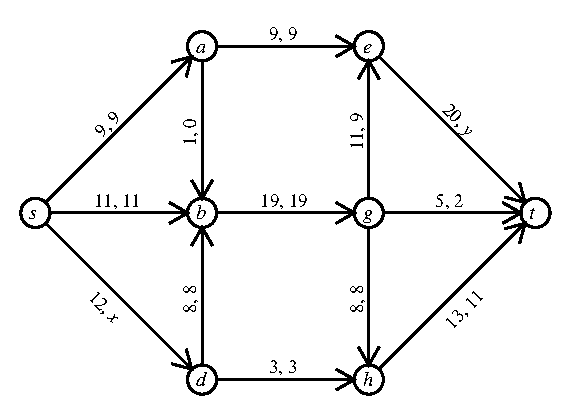
\includegraphics[width=0.6\linewidth]{./figure/g111.pdf}
\caption{グラフ$G_1$}
\label{g111}
\end{figure}

\begin{enumerate}[(a)]
\item $x$, $y$ を求めよ。
\answer{解}
$x = 11, \, y = 18$
\item フロー $f$ の流量 $|f|$ を求めよ。
\answer{解}
$|f| = 31$
\item カット $C=\{(s,a), (b,g), (d,h), (a,b)\}$ の容量を求めよ。なお、$C$ の辺をすべて開放除去すると、$G_1$ は2つの連結成分に分かれる。それらのうち、$s$ を含む方の点の集合を $X$、それ以外の点の集合を $\bar{X}$ とすれば、このカットは $C(X,\bar{X})$ と書くことができる。
\answer{解}
$|C(X,\bar{X})| = 31$
\end{enumerate}

\item 図\ref{g112}の有向グラフ$G_2$について、$s$ から $t$ への最大流問題を考える。
ただし、各辺には、容量 $c$ と現在のフロー $f$ の値がこの順序で記されている。次の各問に答えよ。
\begin{figure}[H]
\centering
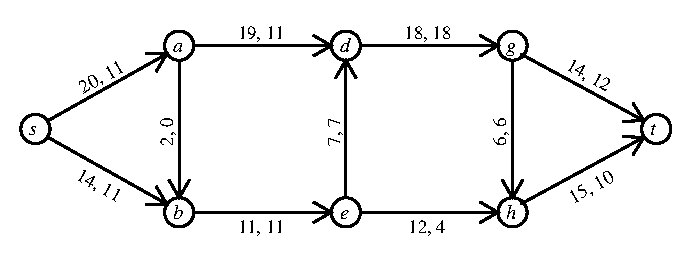
\includegraphics[width=0.5\linewidth]{./figure/g112.pdf}
\caption{グラフ$G_2$}
\label{g112}
\end{figure}
\begin{enumerate}[(a)]
\item 残余グラフ $R(f)$ を求めて図示せよ。
\answer{解}
\begin{figure}[H]
\centering
\includegraphics[width=0.5\linewidth]{./figure/g112a1.pdf}
\caption{残余グラフ$R(f)$}
\label{g112a1}
\end{figure}
\item 増加パス $p$ を求めて図示せよ。ただし、増加パスが複数ある場合には、辺の本数が最も少ないものを選べ。
\answer{解}
\begin{figure}[H]
\centering
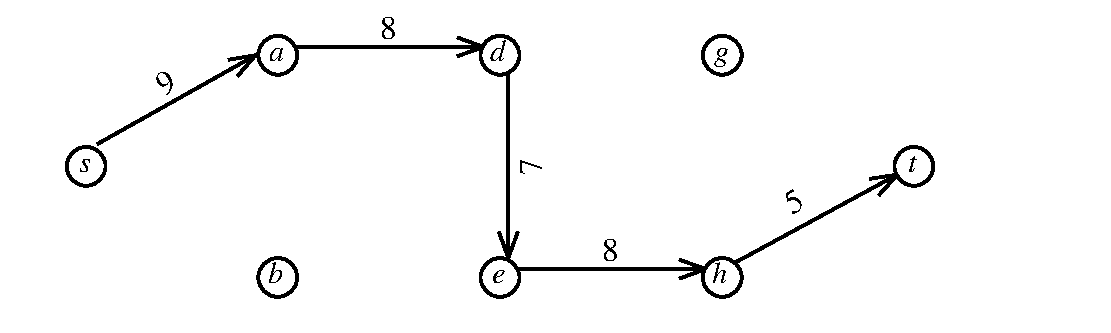
\includegraphics[width=0.5\linewidth]{./figure/g112a2.pdf}
\caption{増加パス$p$}
\label{g112a2}
\end{figure}
\item 上で選んだ増加パス $p$ によって修正されたフロー $f'$ を求めて図示せよ。
\answer{解}
\begin{figure}[H]
\centering
\includegraphics[width=0.5\linewidth]{./figure/g112a3.pdf}
\caption{修正されたフロー$f'$}
\label{g112a3}
\end{figure}

\item 最大フロー $f^*$ を求めて図示せよ。
\answer{解}
\begin{figure}[H]
\centering
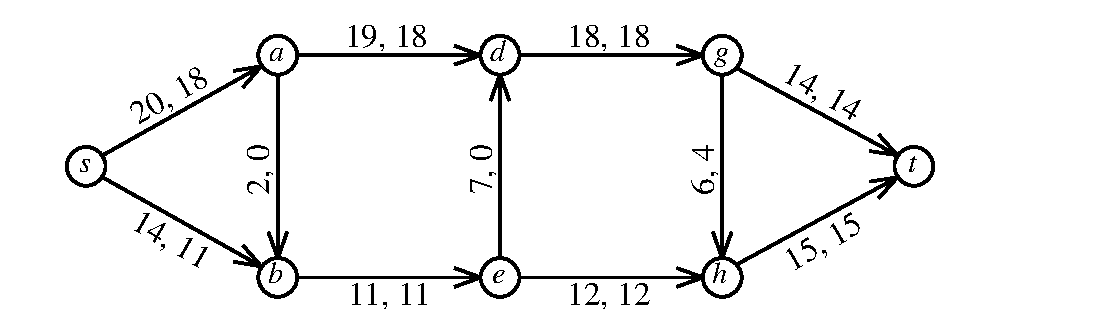
\includegraphics[width=0.5\linewidth]{./figure/g112a4.pdf}
\caption{最大フロー$f^*$}
\label{g112a4}
\end{figure}

\end{enumerate}
\item 最大流をプログラム、MATLABまたはMathematicaで求めよ。
選んだ方法(プログラムの言語またはMATLAB/Mathematica)とスクリーンショットを記すこと。
\begin{enumerate}[(a)]
\item グラフ $G_3$ の点1から11への最大フローを求めよ。得られた最大フローの値、および、最大フローを書き込んだグラフを示せ。
\begin{figure}[H]
\centering
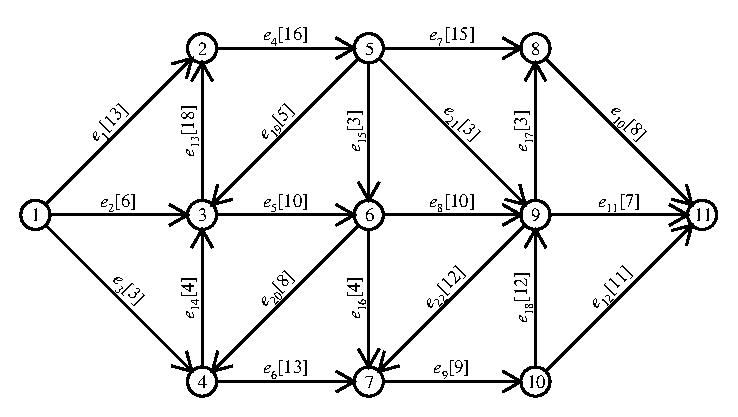
\includegraphics[width=0.6\linewidth]{./figure/g113.pdf}
\caption{グラフ$G_3$}
\label{g113}
\end{figure}
\answer{解}

選んだ方法 Python


最大フローの値 $|f^*| = 8$


最大フロー
\begin{figure}[H]
\centering
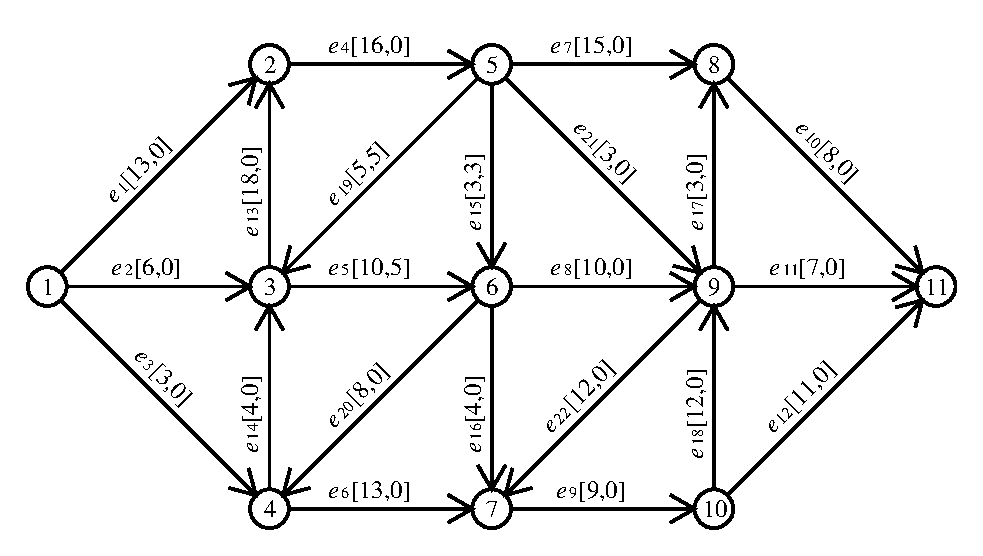
\includegraphics{./figure/g113a.pdf}
\caption{最大フロー}
\label{g113a}
\end{figure}

\begin{figure}[H]
\centering
\includegraphics[width=12cm,height=12cm,keepaspectratio]{./figure/ss11.png}
\caption{スクリーンショット}
\label{g113b}
\end{figure}

\item グラフ $G_4$ の点$v_2$と$v_8$の間の辺連結度$\lambda(v_2,v_8;G)$を求めるための入力を求めよ。
\begin{figure}[H]
\centering
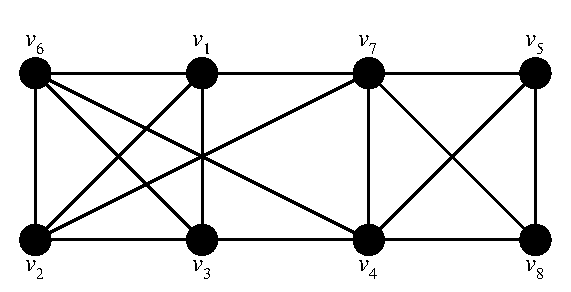
\includegraphics[width=0.6\linewidth]{./figure/g21.pdf}
\caption{グラフ$G_4$}
\label{g113c}
\end{figure}
\answer{解} % 解は\verb| |の中に記す。書き方は言語に合わせて適宜変えること
\begin{itemize}
\item \verb|src= 6,1,7,2,3,4,6,5,1,7,6,2,7,4,4,7,1,7,5,3,4,8,2,8,3,4,3,1,8,5,6,2 |
\item \verb|dst= 1,7,5,3,4,8,2,8,3,4,3,1,8,5,6,2,6,1,7,2,3,4,6,5,1,7,6,2,7,4,4,7 |
\item \verb|cap= 1,1,1,1,1,1,1,1,1,1,1,1,1,1,1,1,1,1,1,1,1,1,1,1,1,1,1,1,1,1,1,1 |
\end{itemize}
\end{enumerate}
\end{enumerate}\newpage
\section*{ミニッツペーパー}
\subsection*{今回の授業内容で重要だと思ったこと}
最大フローについて考える際,残余グラフや増加パスの性質を理解しながら考えることが大切だと感じた.

\subsection*{今回の授業内容でよく理解できなかった点、疑問に思ったこと}
最大流問題と辺連結度の関係性について,証明が難しかった.

%%%%%%%%%%%% 以下、必要に応じて、行頭の%を消去した上で利用してください。
% \section*{謝辞}

%%% urlパッケージを利用できるので、参考文献にWebのURLを記すときには、\url{ }の中に入れてください。
%%% 例) \url{https://en.wikipedia.org/wiki/Complete_graph}
% \begin{thebibliography}{9}
% \bibitem{}
% \end{thebibliography}

%%%%%%%%%%%%

\end{document}

